\section[Abstrakt ]{Abstrakt }



Diese Seminararbeit behandelt das Thema Informationsrückgewinnung und
soll als eine Hilfestellung, für die Umsetzung einer Such-Engine, im
„NoSQL“ Projekt dienen. 

Im Rahmen des „NoSQL“ Projektes wird eine Such-Engine benötigt, die
unstrukturierte Daten in einer Freitextform durchsucht und der Relevanz
entsprechend dem Nutzer auslegt. Um diese fachliche Anforderung zu
implementieren reicht der Key-Value Ansatz, der gängigen Datenbanken,
nicht und muss dementsprechend durch eine andere Umsetzungsform
realisiert werden. In dieser Seminararbeit werden Konzepte und
Verfahren vorgestellt, die eine Volltextsuche sowie die
Relevanzzuordnung der Suchergebnisse ermöglichen. Die entsprechende
Information kann im Buch „Introduction to Information Retrieval“ vom
Christopher D. Manning nachschlagen werden.

Die Seminararbeit beginnt mit der Abgrenzung des Begriff
„Informationsrückgewinnung“, nachfolgend gestalten Verfahren mit
Vorverarbeitungsschritten den Text durchsuchbar und zum Schluss werden
die notwendigen Schritte für die Ergebnisrangliste, der Suchanfrage,
beschrieben. 

Aufbauend auf den vorgestellten Konzepten und Verfahren wird validiert,
ob die Such-Engine {\textquotedbl}Elasticsearch{\textquotedbl} den
Projektanforderungen entspricht.




\section[Einleitung]{Einleitung}



Die zielgerichtete Suche nach Daten wird in der Regel mit einer ID-
Referenz umgesetzt und liefert ein passendes Ergebnis zu dem passenden
Schlüssel. Um eine komplizierte und erfolgreiche SQL Datenbankanfrage
durchzuführen, müssen die Daten sich in einer streng strukturierten
Form befinden. Diese Form ist passend für die Suche über Datensätze wie
Adressen, Produkte und Preise, jedoch ist sie keinesfalls für Daten
unstrukturierter Natur geeignet %
%Ohne Komma, weil kein Verb 
wie zum Beispiel die menschliche Sprache.

Die starke Entwicklung der Hardware, Software und des Internets führen
neue Informationsquellen ein: Blogs, Foren, Wikis, soziale Netzwerke
bis zu den Lernplattformen. Diese modernen Informationsquellen führen
eine große Menge an unstrukturierter Daten ein, die Durchsuchbar
gestaltet werden müssen. Damit ist die Suche über eine große Menge von
Texte in natürlicher Sprache eine zentrale Disziplin. 




Das entschiedene Ziel der Volltextsuche: Das Auffinden und Bewerten der
relevanten Information, die in natürlicher Sprache gespeichert ist,
ohne einen Schlüsselverweis auf den enthaltenen Datensatz. 

Damit die folgende oft unangenehmen Situation nicht mehr auftritt.




„Es tut mir leid, ich kann in Ihre Bestellung nur nachsehen, wenn Sie
mir Ihre Bestellnummer geben können.“




\section[Begriffsklärung]{Begriffsklärung}



Der Begriff Informationsrückgewinnung kann auf unterschiedliche Weise
interpretiert und zu unterschiedlichen Disziplinen zugeordnet werden. 

Die Definition der Informationsrückgewinnung im Kontext der
Volltextsuche kann leicht missverstanden und in Verbindung mit
Datamining gebracht werden. Jedoch dürfen die beiden Disziplinen nicht
mit einander verknüpfen werden, da diese grundsätzlich unterschiedliche
Ziele verfolgen.

Die Informationsrückgewinnung soll im Gegensatz zu Datamining keine
neuen Informationen gewinnen, sondern die vorhandenen, enthaltene
Information soll zugänglich und auffindbar gemacht werden.




\section[Vorbereitung der Lösungsansätze]{Vorbereitung der
Lösungsansätze}



Um die Suchansätze anschaulich darzustellen, wird ein Szenario mit einer
Sammlung von durchsuchbaren Dokument benötigt. Ein Dokument besteht aus
einer Menge von Schlüsselwertpaaren, diese können Strings, Integer und
andere Schlüsselwertpaaren enthalten. Zum Beispiel kann ein
Artikeldokument aus drei Feldern aufgebaut werden, in dem Autor, Titel
und Textkörper enthalten sind, die in sich einen beliebigen Text tragen
können (inklusive Integer, Daten, Weblinks). 

Unser Ziel ist es, aus einer Menge von Dokumenten die in sich
unterschiedliche Strukturen aufweisen dürfen, für den Nutzer relevanten
Dokumenten zu filtern.




\subsection[Lineare Suche]{Lineare Suche}



Der einfachste Weg relevante Information aus einer Datensammlung zu
filtern, ist das Scannen der Dokumente einer Sammlung nach passenden
Suchtermen und das Auslegen der Trefferdokumente als eine
Ergebnisliste. Der lineare Suchansatz kann in viele Bereichen nützlich
sein wie zum Beispiel das Linux „cat“ Funktion, jedoch ist dieser nicht
für alle Systeme und Sammlungen geeignet, denn zusammen mit der
Dokumentenanzahl wächst die Suchzeit proportional mit. 

Somit ist das Suchen in großen Datenmengen, %
%Partizip Gruppe, bezogen auf das Suchen 
besonders im Onlineformat, nicht durchführbar.







\subsection[Matrix Suche]{Matrix Suche}



Da die lineare Suche nur auf kleine Datensätze durchgeführt werden kann,
wird ein anderer Ansatz benötigt, der Arbeit im Voraus leistet, um
später die Suche zu vereinfachen. Es werden gewisse Metainformationen
des gespeicherten Dokumentes in einer Datenstruktur abgelegt, die das
Suchen unterstützen und beschleunigen sollen. 

Diese Struktur ist in einer Häufigkeitsmatrix aufgebaut und speichert
für jedes Wort und Dokument einen Boolean, der auf existieren eines
Wortes im Dokument verweist.

\begin{figure}
\centering
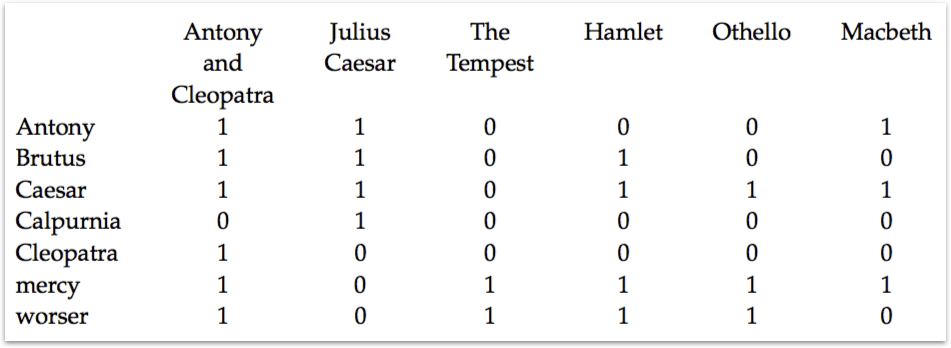
\includegraphics[width=13.54cm,height=4.955cm]{bilder/SeminararbeitArkadij-img1.png}
\end{figure}



In dieser Datenstruktur wird die Suche in einer Boolean-Form
abgearbeitet. Es werden {\textquotedbl}1{\textquotedbl} und
{\textquotedbl}0{\textquotedbl} für jedes Dokument, das einen
bestimmten Such-Term beinhaltet, ausgelesen. Auf diese Weise können
Dokumente auf Existenz einzelner Terme untersucht werden. Ferner könne
die Terme in Kombination mit einander, durch die AND, OR, NOT
Operatoren, verarbeitet werden.




Die Suche nach der Term-Kombination „Brutus ${\wedge}$ Caesar ${\wedge}$
¬Calpurnia“ kann jetzt leicht mit Hilfe der Häufigkeitsmatrix
berechenbar werden. 




110100 AND 110111 AND 101111 = 100100




\subsection[Invertierter Index]{Invertierter Index}



Als ein wesentlicher Nachteil der Häufigkeitsmatrix ist die dominierende
Belegung mit NULL Werten, die keine Relevanz für die Suche darstellen.
Dementsprechend gibt es einen besseren Ansatz mit Häufigkeitslisten,
die für jeden Such-Token eine Liste an Dokumentreferenzen zuweist.
Daraus entstehen auf der rechten Seite ein Wörterbuch und auf der
linken Seite eine Verweisliste. 

\begin{figure}
\centering
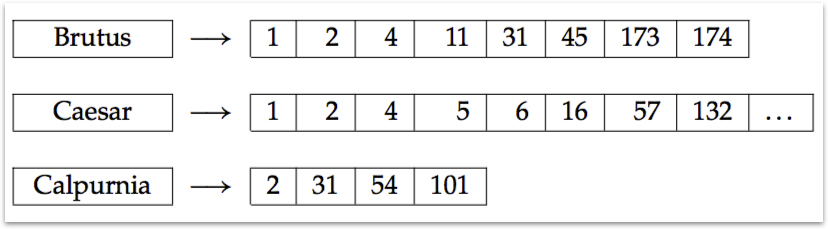
\includegraphics[width=13.143cm,height=3.634cm]{bilder/SeminararbeitArkadij-img2.png}
\end{figure}



Um die Performance der Suche zu steigern, kann die Datenstruktur in sich
geordnet aufgebaut werden, indem das Such-Term-Wörterbuch alphabetisch
und der Listeninhalt nach den Dokumenten ID’s sortiert wird. Eine
weitere Performance Steigerung ergibt sich aus der Datenstruktur, diese
erlaubt die Trennung des Wörterbuches und der Verweislisten auf
unterschiedliche Speichermedien. Dadurch wird das relativ kleine
Wörterbuch im Arbeitsspeicher gehalten und die großen Verweislisten von
der Festplatte bei Bedarf nachgeladen.




\section[Indexaufbau ]{Indexaufbau }


Bevor die Terme in den invertierten Index geladen werden, müssen diese
mehrere Vorverarbeitungsschritte durchlaufen. Die im Text vorkommende
Worte müssen in Terme aufgeteilt, gefiltert, zusammengefasst,
normalisiert und in semantisch äquivalente Gruppen zusammengefasst
werden. Erst wenn die Vorverarbeitung des Dokumentes abgearbeitet ist,
dürfen die Tokens den Index erweitern. 

Für die spätere Suche werden statistische Informationen über das
Dokument, %
%Beginn einer Erläuterung 
wie die Anzahl der Token, mitgespeichert.

Diese Informationen sind für eine Boolean-Suche nicht entscheidend,
dennoch steigern sie die Effizienz der Suchmaschine zur Abfragezeit.

\subsection[Tokenisierung]{Tokenisierung}


Im ersten Schritt wird der Text in Tokens aufgegliedert. Diese
beschreiben ein Wort oder eine Wortmenge, die einen Begriff
widerspiegeln. Dies scheint eine simple Aufgabe zu sein, jedoch hat der
Toknisierung Vorverarbeitungsschritt viele Tücken. 

Namen, Nummern und Daten können von der Norm abweichende Form einnehmen
wie z.B. „O'Neil“, „Loas Anageles“, „Mar 18,1990“,
„(+49)345-3455“ und damit die Tokenisierung erschweren. Trotzdem müssen
die Tokens als eine Einheit erkannt und gespeichert werden. \ 


Zusätzlich bringt die deutsche Sprache eigne Regel, die zusätzlich beim
Tokanisieren beachtet werden müssen. Zum Beispiel muss das Wort
„Lebensversicherungsgesellschaftsangestellter{\textquotedbl} in
eigenständige Einheiten zerlegt und gespeichert werden. Dieser Schritt
bedarf einer komplexen Analysephase und tiefen Verständnis der
deutschen Sprache. 

Zuletzt muss der Kontext der Datensammlung beachtet werden und die
existierenden Trends der Abkürzungen und Darstellungsformen für
bestimmte Ereignisse, Materialen, Werkzeuge und Orte miteinberechnet
werden.

Demzufolge braucht der Tokenisierung-Schritt viel Aufmerksamkeit und
fein Tuning für ein angenehmes Suchverhalten. \ 

\subsection[Filterung]{Filterung}

Nachdem die Tokens gebildet wurden, kann das Filtern beginnen. Es werden
Tokens mit geringem Informationsgehalt wie „der, die, das“ oder in der
englischen Sprache „a, an, and, are, it, be, for, let“ nicht
mitgespeichert, um Ballastinformation zu vermeiden. Damit hätte man den
Speicherverbrauch stark reduziert, da diese Worte fast in jedem
Dokument in großer Anzahl auftreten werden. Allerdings können bei
diesem Sparansatz Nebeneffekte auftreten, die mit Sinn belegte Sätzen,
bestehend aus den Stoppwörtern, rausfiltern: „let it be“. 

\subsection[Normalisierung ]{Normalisierung }


Im nächsten Schritt werden die Terme normalisiert. Es werden Terme mit
gleicher Bedeutung und unterschiedlicher Schreibweise zu einem Term
zusammengefasst. Zum Beispiel erwarten wir für eine Suche nach U.S.A
ein Ergebnis, welches allen Synonymen im Text entspricht (U.S.A == USA
== United Stats of America). 

Damit die Suche Synonyme äquivalent behandelt, müssen diese mit einander
verlinkt werden. Diese Anforderung kann mit Hilfe der Äquivalenzklassen
umgesetzt werden, die die, in der Klasse enthaltenen, Terme
verallgemeinern und übergreifend dieselbe Bedeutung zuweisen.
Andererseits können Abfrageerweiterungslisten erstellt werden, die
flexibel und individuell die Bedeutung der Terme gestalten können.


\subsection[Stemming \& Lemmanisation]{Stemming \& Lemmanisation}

Die übrig gebliebenen Tokens tragen immer noch die Metainformation aus
dem Satzbau wie Zeit und Raum. Diese Information lässt einen Term mit
derselben Bedeutung unterschiedlich erscheinen, demzufolge müssen die
Terme auf eine gemeinsame Grundform zurückgeführt werden. 


Es gibt zwei Ansätze dies umzusetzen. Im ersten Ansatz „Lemmatisierung“
werden die Worte auf einen gemeinsamen Stamm zurückgeführt. Zum
Beispiel werden die Worte „liefen“, „laufend“, „gelaufen“ auf den Stamm
„laufen“ zurückgeführt. Dies mag eine passende Umsetzung für zahlreiche
Sprachen sein, jedoch verliert dieser Ansatz an Bindung von Worten mit
starker Ähnlichkeit wie z.B. \ das englische Wort „operating“ mit dem
Stamm “operate“ kann nicht auf “operational“ oder „operative“
zurückgeführt werden. Demzufolge wird oft der „Stamming“ Ansatz
angewandt. Dieser trimmt die Endung eines Wortes, sodass nur die Basis
des Wortes für die Indexierung genutzt wird. Somit werden die Worte
„operating“ und “operational“ passend auf den Term „operat“
runtergebrochen.

Dokument Rangliste

\subsection{}
Bis lang wurden Konzepte der Datenstrukturen sowie der Vorverarbeitung
vorgestellt, diese bereinigen den Text vor unnötigen Information,
fassen gemeinsame Terme zusammen und speichern diese in einer für die
Suche optimalen Datenstruktur. Obwohl die Suche saubere Ergebnisse
liefert, können die Ergebnisse nicht auf Relevanz untersucht werden. \ 

In diesem Kapitel werden die fehlenden Konzepte zur Durchführung der
Bewertung der Suchergebnisse vorgestellt.

\subsection[Dokumenten{}-Zonen]{Dokumenten-Zonen}


Das Dokument besteht aus mehreren Bereichen, diese beinhalten Terme, die
unterschiedlich gewichtet werden können, wie zum Beispiel Titel,
Textkörper und Anhang. Mit Hilfe dieser Information wird eine Ordnung
der gefundenen Dokumente erstellt und nur die wesentlichen als Ergebnis
ausgelegt.


Beispielsweise wird für jeden Term ein Tupel in der Referenzliste
erstellt, das nicht nur auf das enthalte Dokument, sondern auch auf den
zugehörigen Bereich verweist. 


[Willy]-{\textgreater} [2, Autor, Titel] [3, Anhang] [45, Textkörper]

Da die Bereiche nicht gleich wichtig sind, werden diesen Gewichte
zugewiesen, sodass sie zusammen 1 ergeben. Bei der Suche wird das
Dokument nach dem Such-Termen durchforschtet und anschließend ein
Ranking erstellt, indem die Summe der Gewichte über alle Zonen des
Dokumentes gebildet wird. 

\begin{figure}
\centering
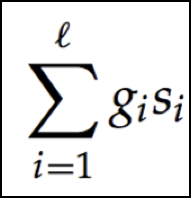
\includegraphics[width=3.381cm,height=3.507cm]{bilder/SeminararbeitArkadij-img3.png}
\end{figure}



Obwohl es eine sinnvolle Umsetzung ist, mangelt dieser an Domäne Wissen
über die einzelnen Zonen, somit muss das Gewicht für jede Zone manuell
eingetragen werden. Dies ist möglich mit Hilfe eines Experten oder
einem maschinellen Lernverfahren über eine große Datenmenge, jedoch
gibt es bessere Alternativen. 

\subsection[Document Term Frequency DTF]{Document Term Frequency DTF}

Bislang wird die Bewertung eines Dokumentes über eine Term-
Existenzabfrage erstellt. In den nächsten Schritt wird diese Logik
erweitert: Ein Dokument oder eine Zone, die einen Abfragebegriff
häufiger erwähnt hat mehr mit dieser Abfrage zu tun und sollte daher
eine höhere Wertung erhalten.

Damit bekommt jeder Term in einem Dokument ein Gewichtsfaktor, der von
der Anzahl an Vorkommen von diesem Term im Dokument abhängt. Dieser
heißt „Document Term Frequency“ oder „DTF“ [tf (t,d)]. 

Für den Term „Willy“ könnte eine Referenzliste diese Form einnehmen.


[Willy]-{\textgreater} [25, Author \{6\}, Title \{25\}] [75, Title
\{7\}]

Der vorgestellte Ansatz liefert genauere Ergebnisse, nicht desto trotz
könne die Suchergebnisse überraschen, denn nicht jedes Wort ist gleich
wichtig allen anderen Wörtern. 


\subsection[Inverse Document Frequency IDF]{Inverse Document Frequency
IDF}

Der IDF bezweckt eine bessere Bewertung des Informationsgehalts eines
Terms, denn häufig auftretende Worte innerhalb einer Sammlung haben
eine mangelhafte Aussagekraft und schränken den Suchbereich nicht ein.
Also müssen Worte, die selten auftreten, höher priorisiert werden als
Worte, die in jedem Dokument in großer Anzahl auftreten. Damit würden
oft auftretenden Terme die Suche nicht in die falsche Richtung
verzehren. 




Um das geplante Verhalten zu erzeugen wird eine Formel verwendet, die
ein Verhältnis von der Gesamtheit aller Dokumente zu den Dokumenten mit
dem entsprechenden Term aufstellt.

Wenn die Gesamtzahl der Dokumente in einer Sammlung mit „N“ bezeichnet
wird und die Anzahl an Dokumenten, in denen ein Term „t“ auftaucht
„DTF“, wird die inverse Dokumenthäufigkeit „IDF“ eines Terms „t“ wie
folgt definiert: 

\begin{equation*}
\mathit{IDF}\left(t\right)={\log
}_{10}\left(\frac{N}{\mathit{DTF}}\right)
\end{equation*}



Desto weniger Dokumente mit dem entsprechenden Term in der Sammlung
existiert, desto größer der IDF und desto wichtiger die Ergebnisse.

IDF hat keine Auswirkung auf Abfragen mit einem einzelnen Term, wenn
dieser drin ist sind alle Dokumente gleichwertig.


\subsection[TF{}-IDF]{TF-IDF}
Jetzt kann die Definitionen von Dokument-Term-Häufigkeit DTF in
gegebenen Dokument und die inversem Dokumentenhäufigkeit IDF für den
Term kombiniert werden, um ein zusammengesetztes Gewicht für jeden Term
in jedem Dokument zu erzeugen.

Das TF-IDF-Gewichtungsschema weist dem Term t eine Gewichtung in
Dokument d zu, gegeben durch:


\begin{equation*}
\mathit{TF}.\mathit{IDF}=\mathit{TF}{\ast}\mathit{IDF}
\end{equation*}



Mit Hilfe des TF-IDF kann das Ranking eines Dokumentes für eine gegebene
Abfrage berechnet werden. Es werden TF-IDF‘s für jeden Term, der sowohl
in der Abfrage als auch im Dokument enthalten ist, berechnet und
summiert.

Somit entsteht eine Relevanzeinschätzung für eine gegebene Abfrage und
Dokument aus der Sammlung.

\begin{figure}
\centering
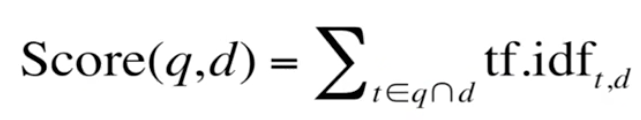
\includegraphics[width=9.821cm,height=1.838cm]{bilder/SeminararbeitArkadij-img4.png}
\end{figure}

Sobald für jedes Dokument der TF-IDF berechnet und in die Inzidenzmatrix
eingesetzt wurde, entsteht eine Gewichtsmatrix.

Mit Hilfe dieser, kann anhand des Dokumentenvektors ablesen werden, wie
wichtig eine Abfrage ist, indem alle vorkommen von gesuchten Termen
zusammenlegt werden.


\begin{figure}
\centering
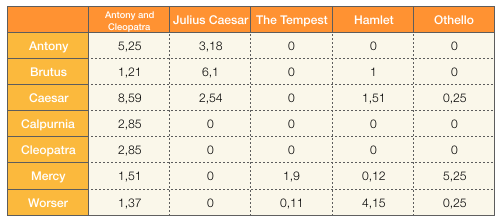
\includegraphics[width=13.208cm,height=5.854cm]{bilder/SeminararbeitArkadij-img5.png}
\end{figure}

\subsection[Vector Space Model ]{Vector Space Model }

Im letzten Kapitel wurden Methoden vorgestellt, wie die Dokumente in
Vektoren umgewandelt werden können, jedoch gibt es andere
Datenstrukturen, die das Erstellen des Rankings signifikant
beschleunigen können.

Das Vektormodel beschreibt ein V-Dimensionalen Vektorraum, wobei V die
Anzahl an Termen darstellt. Die Achsen des Vektorraum werden durch alle
existierenden Terme repräsentiert, die im späteren Verlauf mit der
Suchanfrage abgeglichen werden

Die Ähnlichkeit der Suchanfrage könnte über die euklidische Distanz des
Abfrage-Punkt sowie der Vektorraum-Punkte berechnet werden. Jedoch
würden Dokument, die sehr viel mit der Suchanfrage zu tun haben, sich
mit jedem Vorkommen an relevanten Termen von dem Abfrage-Punkt
entfernen. In der folgenden Abbildung besitzt ein Dokument die nötigen
Begriffe zweimal und hat damit die doppelte Entfernung vom Nullpunkt.


\begin{figure}
\centering
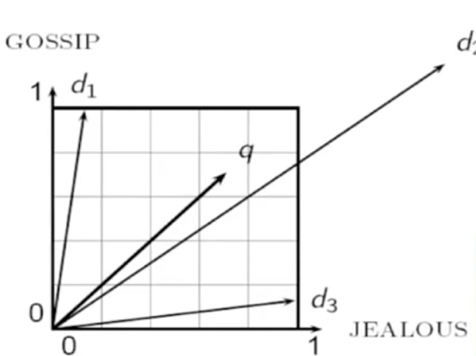
\includegraphics[width=6.435cm,height=4.81cm]{bilder/SeminararbeitArkadij-img6.png}
\end{figure}


Dementsprechend sollte die euklidische Distanz nicht für die
Ähnlichkeitsberechnung der Vektoren genutzt werden und wird im
Folgenden vom winkelbasierten Ansatz abgelöst. 

Beim winkelbasierten Ansatz wird die Länge der Vektoren im Vektorraum
und die Länge des Abfragevektors normalisiert und anschließend mit
Hilfe der Cosine-Similarity auf Ähnlichkeit abgeglichen.

Dabei werden Winkel zwischen der Abfrage und den Dokumenten aus der
Sammlung berechnet und Dokumente mit einer ähnlichen Ausrichtung als
Ergebnisliste zurückgegeben.


\begin{figure}
\centering
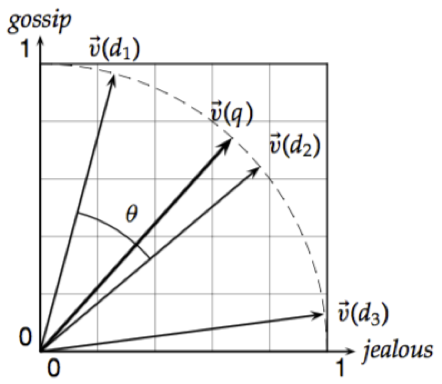
\includegraphics[width=6.361cm,height=5.528cm]{bilder/SeminararbeitArkadij-img7.png}
\end{figure}


Diese Vorgehnesweise zur berechnung der Ähnlichket von zwei Vektoren
wird wie schon beschrieben durche eine Normalisierung wie Verschmelzung
der bedien Vektoren berechnet.



\begin{figure}
\centering
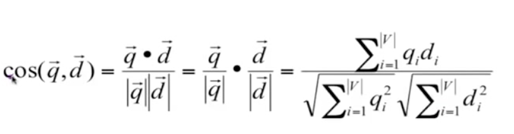
\includegraphics[width=9.465cm,height=2.466cm]{bilder/SeminararbeitArkadij-img8.png}
\end{figure}


\subsection[Schluss]{Schluss}

Ist eine Such-Engine die mit Volltextsuche ausgestattet ist ausreichend
für die Suche nach Textbausteinen aus einer Menge von Dokumenten? Ja,
das ist sie. Die vorgestellten Modelle zum Abspeichern von Daten in
einer Freitextform ermöglicht das Suchen nach Term-Kombinationen in
einer Datenmenge. Zusätzlich kann mit Hilfe der Metainformation des
Dokumentes wie der Sammlung Ranglisten erstellt werden, die relevante
Dokumente höher priorisieren. 

Für die Umsetzung des Datenmodells können Referenzlisten oder
Inzidenzmatrix genutzt werden. \ 

Für die Umsetzung der Ranglisten werden Metainformation der Sammlung,
wie der einzelner Dokumente verwendet, um bestimmte Verhältnisse
erstellen zu können.

